\documentclass[aspectratio=169]{beamer}

\usetheme{Madrid}
\usecolortheme{DSLAB}
\usefonttheme[onlylarge]{structurebold}
\setbeamerfont*{frametitle}{size=\normalsize,series=\bfseries}
\setbeamertemplate{navigation symbols}{}

\usepackage[utf8]{inputenc} 
\usepackage[T1]{fontenc}
\usepackage[english]{babel}
\usepackage{xmpmulti}
\usepackage{tikz}
\usepackage{pgf}
\usepackage{amsmath}
\usepackage{amsfonts}
\usepackage{graphicx}
\usepackage{color}
\usepackage{multirow}
\usepackage{lmodern}
\usepackage{hyperref}
\usepackage{eurosym}
\usepackage{listings}

\lstset{
  basicstyle=\ttfamily\small,
  frame=single,
  breaklines=true,
  showstringspaces=false,
  columns=fullflexible
}


\usetikzlibrary{arrows}
\tikzstyle{block}=[draw opacity=0.7,line width=1.4cm]

\setbeamercovered{dynamic}
\setbeamerfont{author}{family=\rmfamily}
\institute[URJC]{DSLAB}

\author[Big Data Processing II]{
	Alberto Fernández Isabel \\
	Natalia Madrueño Sierro \\
	Rubén Rodríguez Fernández \\
}

\title[Presentación]{
	Big Data Processing II \\ \vspace{0.2em}
	IA Generativa aplicada al deporte \\ \vspace{0.2em}
    Prompt Engineering \& Post-training
}
\date{Marzo 2026}
\titlegraphic{
\includegraphics[width=3cm]{images/logos/logourjceps.png}}


\setbeamertemplate{section page}{
	\vspace{1cm}
	\begin{beamercolorbox}[sep=8pt,center,wd=\textwidth]{section title}
		\usebeamerfont{section title}\insertsection\par 
	\end{beamercolorbox}
}

% =====================================================
\begin{document}

\begin{frame}
\titlepage
\end{frame}

%------------------------------------------------
\section{Mapa del bloque}
\frame{\sectionpage}

\begin{frame}{Arquitectura conceptual del bloque}
\begin{center}
\Large
\begin{tabular}{c}
{\color{colorblue}\textbf{Sesión 1}} \\ 
{\color{colorblue}Control del comportamiento} \\
{\color{colorblue}\small Prompt Engineering + Post-training}
\\[0.1em]
$\Downarrow$
\\[0.1em]
{\color{gray2}\textbf{Sesión 2}} \\ 
{\color{gray2}Control de la información} \\
{\color{gray2}\small Retrieval-Augmented Generation (RAG)}
\\[0.1em]
$\Downarrow$
\\[0.1em]
{\color{gray2}\textbf{Sesión 3}} \\ 
{\color{gray2}Control del flujo y la acción} \\
{\color{gray2}\small Agentes, Tools y Arquitecturas Cognitivas}
\end{tabular}
\end{center}
\end{frame}

% =====================================================
\section{Contexto}
\frame{\sectionpage} 

\begin{frame}\frametitle{Objetivos de la sesión}
\begin{itemize}
    \item Entender qué es un LLM desde el punto de vista computacional.
    \item Comprender su papel en la Ciencia de Datos Deportivos.
    \item Aprender a controlar su comportamiento mediante Prompt Engineering.
    \item Identificar límites del prompting.
\end{itemize}
\end{frame}

\begin{frame}\frametitle{¿Qué es realmente un LLM?}
\begin{columns}[T]
\column{0.5\textwidth}
\begin{itemize}
    \item Modelo probabilístico de generación de texto.
    \item Aprende patrones lingüísticos.
    \item Predice la siguiente palabra dada una secuencia.
    \item Simula coherencia, no conocimiento real.
\end{itemize}

\column{0.5\textwidth}
\centering
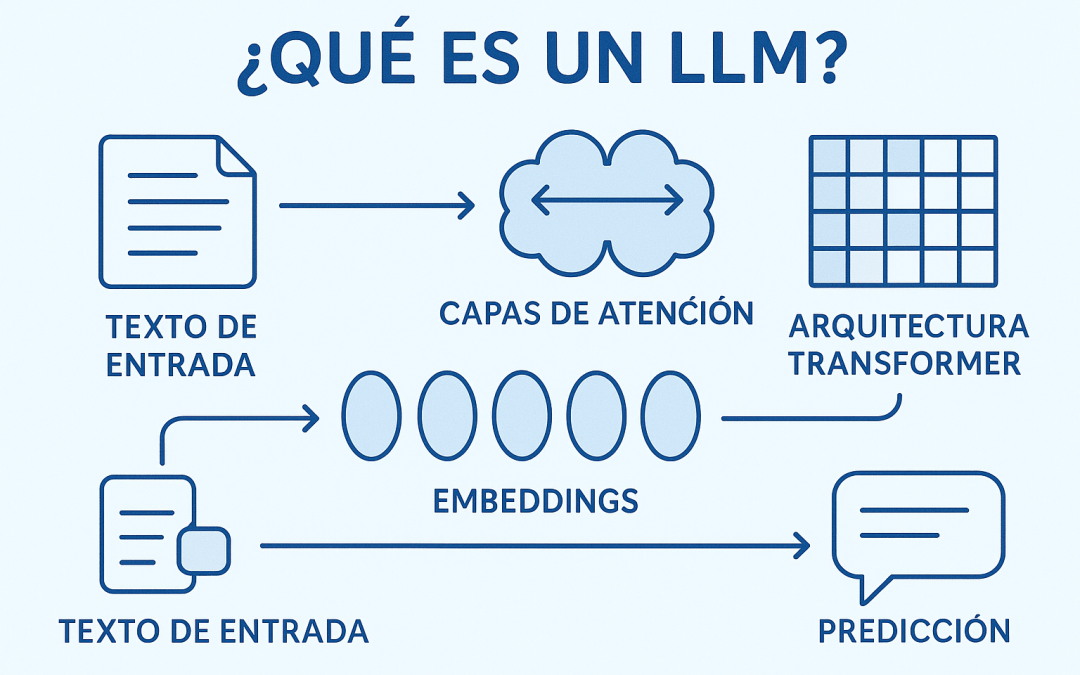
\includegraphics[width=0.9\textwidth]{images/presentacion/transforrmer.png}
\end{columns}
\end{frame}

\begin{frame}\frametitle{Qué NO es un LLM}
\begin{columns}[T]
\column{0.5\textwidth}
\begin{itemize}
    \item \textbf{No es una base de datos}.
    \item \textbf{No tiene acceso} a sensores o APIs.
    \item \textbf{No realiza cálculos fiables} por sí mismo.
    \item \textbf{No distingue verdad de plausibilidad}.
\end{itemize}

\column{0.5\textwidth}
\centering
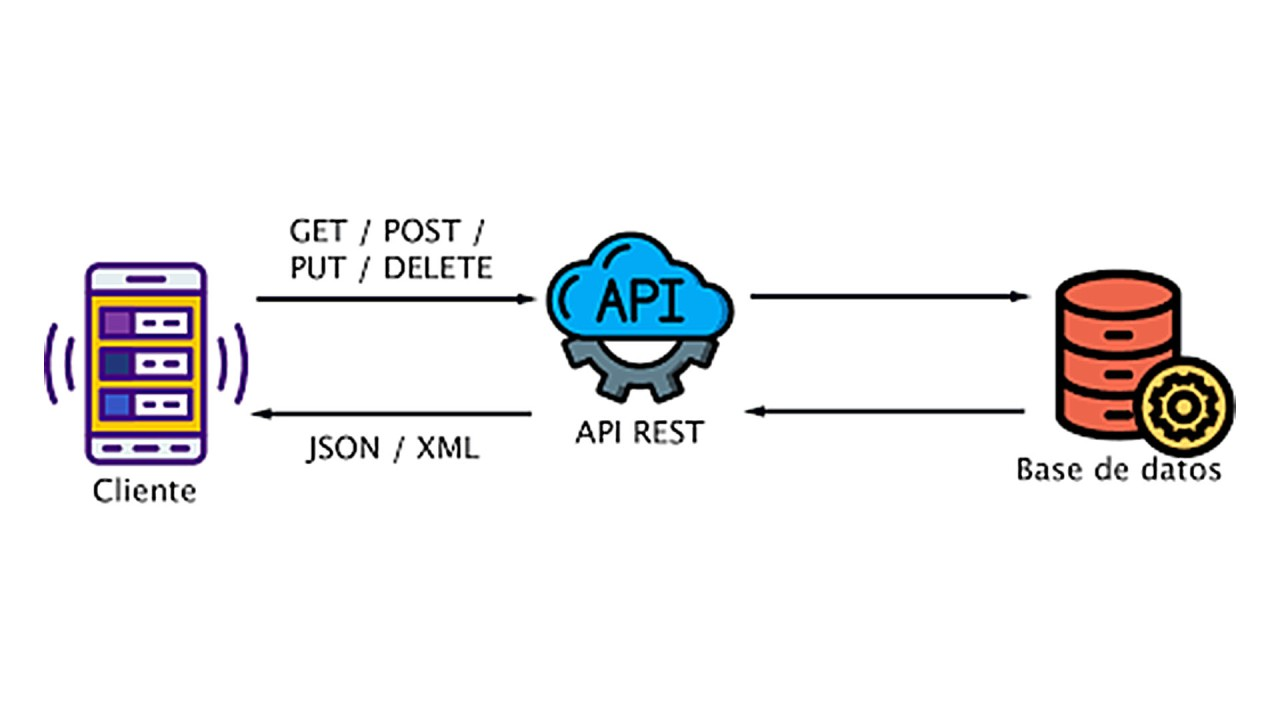
\includegraphics[width=0.8\textwidth]{images/presentacion/bbdd.jpg}
\end{columns}
\end{frame}

\begin{frame}\frametitle{Rol del LLM en analítica deportiva}
\begin{columns}[T]
\column{0.5\textwidth}
\begin{itemize}
    \item Generar narrativas.
    \item Estandarizar informes.
    \item Traducir estadísticas a lenguaje humano.
    \item Interfaz conversacional.
\end{itemize}

\column{0.5\textwidth}
\centering
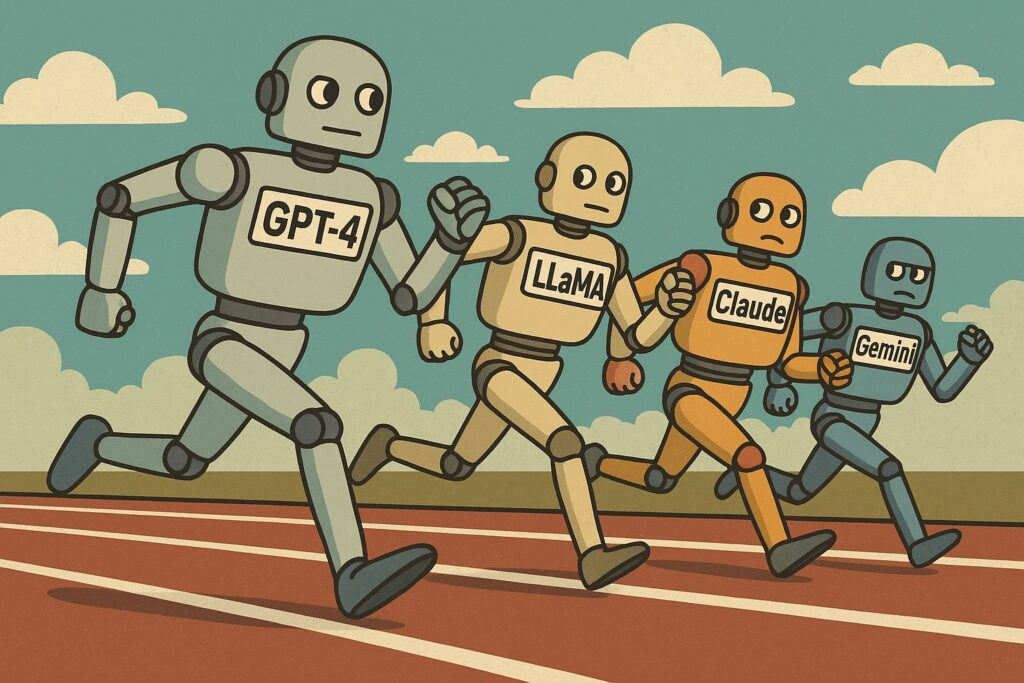
\includegraphics[width=0.8\textwidth]{images/presentacion/carrera.jpg}
\end{columns}
\end{frame}

% =====================================================
\section{Prompt Engineering}
\frame{\sectionpage}

\begin{frame}\frametitle{Prompt = interfaz de control del modelo}

Un LLM no se “usa”, se \textbf{configura mediante lenguaje}.

\vspace{0.4em}

\begin{itemize}
    \item El prompt es el mecanismo con el que definimos:
    \begin{itemize}
        \item Qué tarea debe realizar.
        \item Qué información puede usar.
        \item Qué formato debe producir.
    \end{itemize}

    \vspace{0.3em}

    \item En un sistema de datos, el prompt actúa como:
    \begin{itemize}
        \item Capa de control sobre el comportamiento del modelo.
        \item Sustituto de una interfaz de programación tradicional.
    \end{itemize}

    \vspace{0.3em}

    \item El modelo no cambia internamente → solo cambia su comportamiento en esa interacción.
\end{itemize}

\vspace{0.3em}
\textbf{Idea clave:} Prompt Engineering = programación en lenguaje natural.
\end{frame}


\begin{frame}\frametitle{Preguntar vs especificar una tarea}

Un error común es tratar al LLM como si fuera un buscador o una persona.

\vspace{0.4em}

\begin{itemize}
    \item \textbf{Pregunta informal:}
    \begin{quote}
    “Resume el partido de ayer.”
    \end{quote}
    \begin{itemize}
        \item Ambigua.
        \item Sin contexto.
        \item Sin criterio de calidad.
    \end{itemize}

    \vspace{0.4em}

    \item \textbf{Especificación de tarea:}
    \begin{quote}
    “Genera un resumen técnico de máximo 5 líneas usando SOLO las métricas dadas.  
    Estructura: contexto, acciones clave, impacto táctico.”
    \end{quote}
\end{itemize}

\vspace{0.4em}
\textbf{Diferencia fundamental:}  
Las preguntas producen texto.  
Las especificaciones producen resultados utilizables en un sistema.
\end{frame}

\begin{frame}
\frametitle{Componentes de un prompt de calidad}

Un prompt profesional no es una frase, es una estructura:

\vspace{0.4em}

\begin{itemize}
    \item \textbf{Rol (Role)}  
    Define el perfil desde el que debe responder el modelo.  
    Ej.: “Eres analista de rendimiento en un club profesional”.

    \vspace{0.3em}

    \item \textbf{Tarea (Task)}  
    Especifica exactamente qué debe hacer.  
    Ej.: “Genera un informe técnico del jugador X”.

    \vspace{0.3em}

    \item \textbf{Contexto (Context)}  
    Información disponible para realizar la tarea.  
    Ej.: estadísticas, partido, periodo, posición del jugador.

    \vspace{0.3em}

    \item \textbf{Restricciones (Constraints)}  
    Limita el comportamiento del modelo.  
    Ej.: “No inventes datos”, “Usa solo las métricas dadas”.

    \vspace{0.3em}

    \item \textbf{Formato de salida (Output Format)}  
    Cómo debe entregarse la respuesta.  
    Ej.: JSON, tabla, bullets, informe estructurado.
\end{itemize}

\vspace{0.4em}
\textbf{Idea clave:} un buen prompt reduce grados de libertad del modelo.
\end{frame}


\begin{frame}\frametitle{Ejemplo mal diseñado (por qué falla)}
\textbf{Prompt:} \textit{“Analiza el rendimiento del jugador.”}
\vspace{0.5em}

\begin{itemize}
    \item \textbf{Ambigüedad de objetivo:} ¿rendimiento ofensivo, defensivo, físico, táctico?
    \item \textbf{Sin contexto:} no hay periodo (partido, mes, temporada) ni rival ni rol.
    \item \textbf{Sin datos:} el modelo tenderá a \textbf{inventar} métricas o asumirlas.
    \item \textbf{Sin criterio:} no defines qué significa “bueno/malo” (percentiles, umbrales).
    \item \textbf{Sin formato:} imposible integrar la salida en un pipeline (ETL/dashboard).
\end{itemize}

\vspace{0.3em}
\textbf{Diagnóstico Big Data:} prompt mal definido = salida no reutilizable + riesgo alto de alucinación.
\end{frame}

\begin{frame}\frametitle{Ejemplo mejorado (control con rol + contexto + restricciones)}
\textbf{Prompt (plantilla):}
\begin{itemize}
    \item \textbf{Rol:} “Eres analista de rendimiento en un club profesional”.
    \item \textbf{Tarea:} “Genera un informe técnico del jugador X”.
    \item \textbf{Contexto:} “Usa SOLO las métricas proporcionadas (tabla adjunta)”.
    \item \textbf{Restricciones:} “No inventes datos; si falta una métrica, marca \texttt{null}”.
    \item \textbf{Formato:} “Devuelve JSON con: resumen, puntos fuertes, puntos débiles, alertas”.
\end{itemize}

\vspace{0.4em}
\textbf{Efecto:} reduces grados de libertad y conviertes la interacción en una “especificación”.
\end{frame}

\begin{frame}\frametitle{Ejemplo deportivo completo (entrada mínima de datos)}
\textbf{Entrada (ejemplo):} métricas por 90 minutos (últimos 5 partidos)
\vspace{0.3em}

\begin{itemize}
    \item \texttt{minutes=432, goals=2, assists=1, xG=1.6, xA=0.9}
    \item \texttt{shots\_p90=2.8, key\_passes\_p90=1.7, passes\_acc=84\%}
    \item \texttt{pressures\_p90=14.2, tackles\_p90=1.1, interceptions\_p90=0.8}
    \item \texttt{distance\_km=10.9, sprints=21, high\_intensity\_runs=52}
\end{itemize}

\vspace{0.4em}
\textbf{Nota:} esto es intencionalmente “poco” para forzar que el prompt gestione faltantes sin inventar.
\end{frame}

\begin{frame}[fragile]\frametitle{Salida esperada en formato estructurado (JSON “pipeline-ready”)}
\textbf{Objetivo:} que la salida sea consumible por procesos automáticos (API/ETL/dashboard)

\vspace{0.4em}
\footnotesize
\begin{lstlisting}
{
  "player": "X",
  "period": "last_5_matches",
  "summary": "... (3-5 lineas)",
  "strengths": ["...", "..."],
  "weaknesses": ["...", "..."],
  "alerts": [{"type":"fatigue_risk","evidence":"..."}],
  "metrics_used": ["minutes","xG","xA","pressures_p90"],
  "missing_metrics": ["duels_won_pct","progressive_passes_p90"]
}
\end{lstlisting}
\normalsize

\vspace{0.2em}
\textbf{Clave:} el modelo no “se luce”; produce un contrato de datos.
\end{frame}

\begin{frame}\frametitle{Por qué el formato estructurado es crítico en Big Data}
\begin{itemize}
    \item \textbf{Trazabilidad:} puedes auditar qué campos rellena y cuáles faltan.
    \item \textbf{Evaluación automática:} validación de esquema (JSON schema), checks.
    \item \textbf{Integración:} dashboard/BI, storage, pipelines batch/stream.
    \item \textbf{Reproducibilidad:} mismo prompt + mismos datos $\rightarrow$ salida comparable.
    \item \textbf{Mitigación de alucinación:} forzar \texttt{null}/\texttt{unknown} evita inventar.
\end{itemize}

\vspace{0.3em}
\textbf{Regla de oro:} si lo vas a usar en un sistema, \textbf{no pidas texto libre}.
\end{frame}

\begin{frame}\frametitle{Prompt como contrato (y por qué versionarlo)}
\begin{itemize}
    \item Un prompt operativo funciona como un \textbf{contrato} entre:
    \begin{itemize}
        \item \textbf{Entrada} (datos disponibles) y \textbf{Salida} (estructura/criterios).
        \item \textbf{Responsabilidades} del modelo (qué puede inferir vs qué no).
    \end{itemize}
    \item En un proyecto real debes:
    \begin{itemize}
        \item \textbf{Versionar} prompts (v1, v1.1...) igual que código.
        \item Registrar: modelo, temperatura, prompt, y cambios de esquema.
        \item Mantener tests con ejemplos (golden set) para evitar regresiones.
    \end{itemize}
\end{itemize}

\vspace{0.3em}
\textbf{Puente a técnicas:} para consistencia, entra Zero/One/Few-shot.
\end{frame}

\begin{frame}\frametitle{Eficiencia: claridad > longitud (y coste en tokens)}
\begin{itemize}
    \item Un prompt largo no es “mejor”: puede introducir contradicciones o ruido.
    \item Buen prompt = \textbf{instrucciones cortas + estructura + ejemplos mínimos}.
    \item Coste típico en sistemas: tokens (entrada + salida) $\Rightarrow$ dinero + latencia.
    \item Estrategia práctica:
    \begin{itemize}
        \item Plantillas reutilizables.
        \item Contexto \textbf{solo} necesario.
        \item Ejemplos (few-shot) compactos.
        \item Formato fijo para minimizar longitud de salida.
    \end{itemize}
\end{itemize}

\vspace{0.3em}
\textbf{Mensaje para el máster:} Prompt engineering también es \textbf{optimización de sistema}.
\end{frame}


% =====================================================

\section{Técnicas de prompting}
\frame{\sectionpage} 

\begin{frame}\frametitle{Zero-shot prompting}
\begin{itemize}
    \item El modelo resuelve la tarea solo con instrucciones.
    \item Se apoya en su conocimiento general aprendido en pretraining.
    \item Ventajas:
    \begin{itemize}
        \item Bajo coste en tokens.
        \item Rápido de diseñar.
        \item Flexible ante tareas variadas.
    \end{itemize}
    \item Limitaciones:
    \begin{itemize}
        \item Menor consistencia de formato.
        \item Más variabilidad en la respuesta.
    \end{itemize}
\end{itemize}
\end{frame}

\begin{frame}\frametitle{Ejemplo zero-shot en deporte}
\textbf{Tarea:} Clasificar tipo de evento táctico.

\textbf{Prompt:}
\begin{quote}
“Clasifica el siguiente evento como: transición ofensiva, ataque posicional o contraataque:  
‘Recuperación en campo propio, pase largo al espacio, finalización en 8 segundos.’”
\end{quote}

\textbf{Observación:} funciona, pero puede variar la explicación y formato.
\end{frame}

\begin{frame}\frametitle{One-shot prompting}
\begin{itemize}
    \item Se añade un ejemplo de entrada–salida correcta.
    \item El modelo imita patrón, estructura y nivel de detalle.
    \item Útil para:
    \begin{itemize}
        \item Informes de scouting.
        \item Clasificaciones consistentes.
        \item Resúmenes con plantilla fija.
    \end{itemize}
\end{itemize}
\end{frame}

\begin{frame}\frametitle{Ejemplo one-shot aplicado a informes}
\textbf{Ejemplo dado al modelo:}

Entrada: métricas de un jugador.  \\
Salida: informe estructurado con fortalezas, debilidades y alerta física. \\

Luego se pide lo mismo para otro jugador.

\textbf{Efecto:} se estandariza la estructura sin entrenar el modelo.
\end{frame}

\begin{frame}\frametitle{Few-shot prompting}
\begin{columns}[T]
    \column{0.5\textwidth}
    \begin{itemize}
        \item Varios ejemplos refuerzan el patrón deseado.
        \item Reduce ambigüedad semántica.
        \item Mejora estabilidad del formato.
        \item Especialmente útil cuando:
        \begin{itemize}
            \item hay terminología técnica
            \item la tarea es subjetiva (evaluaciones)
        \end{itemize}
    \end{itemize}
    \column{0.5\textwidth}
    \centering
    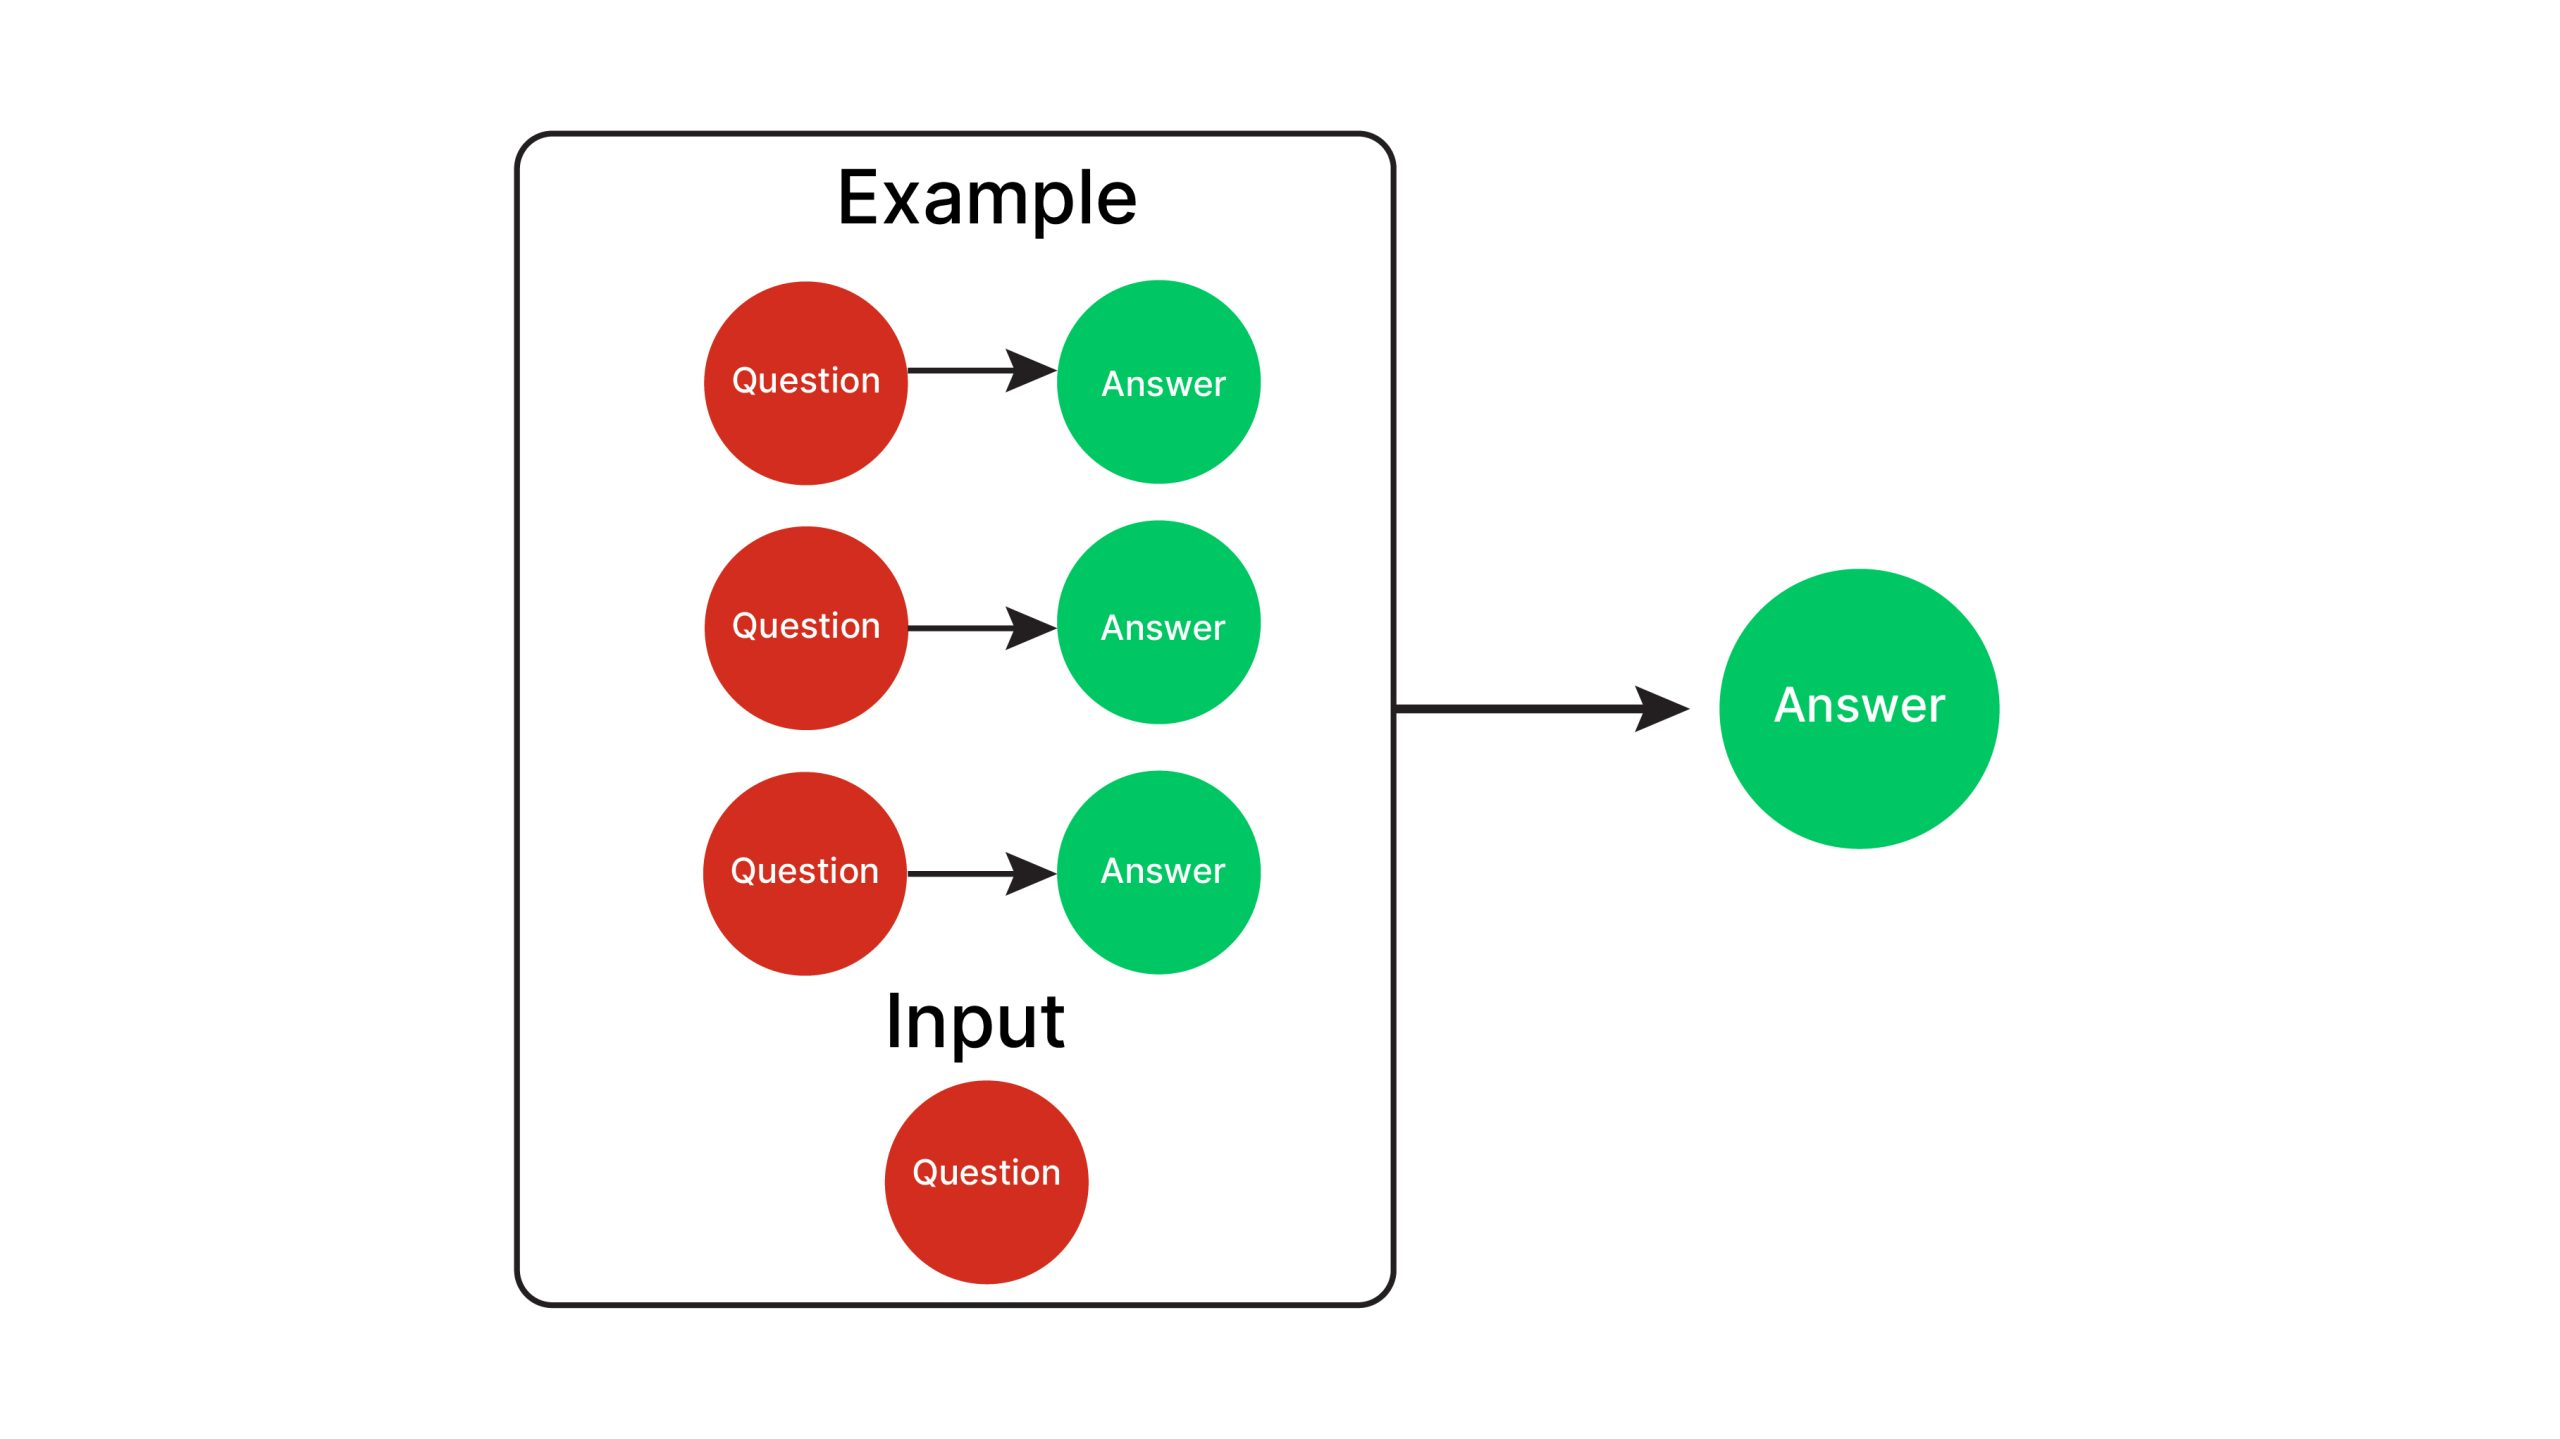
\includegraphics[width=0.8\textwidth]{images/presentacion/fewshot.jpg}
\end{columns}
\end{frame}

\begin{frame}\frametitle{Comparativa Zero vs Few-shot}
\centering
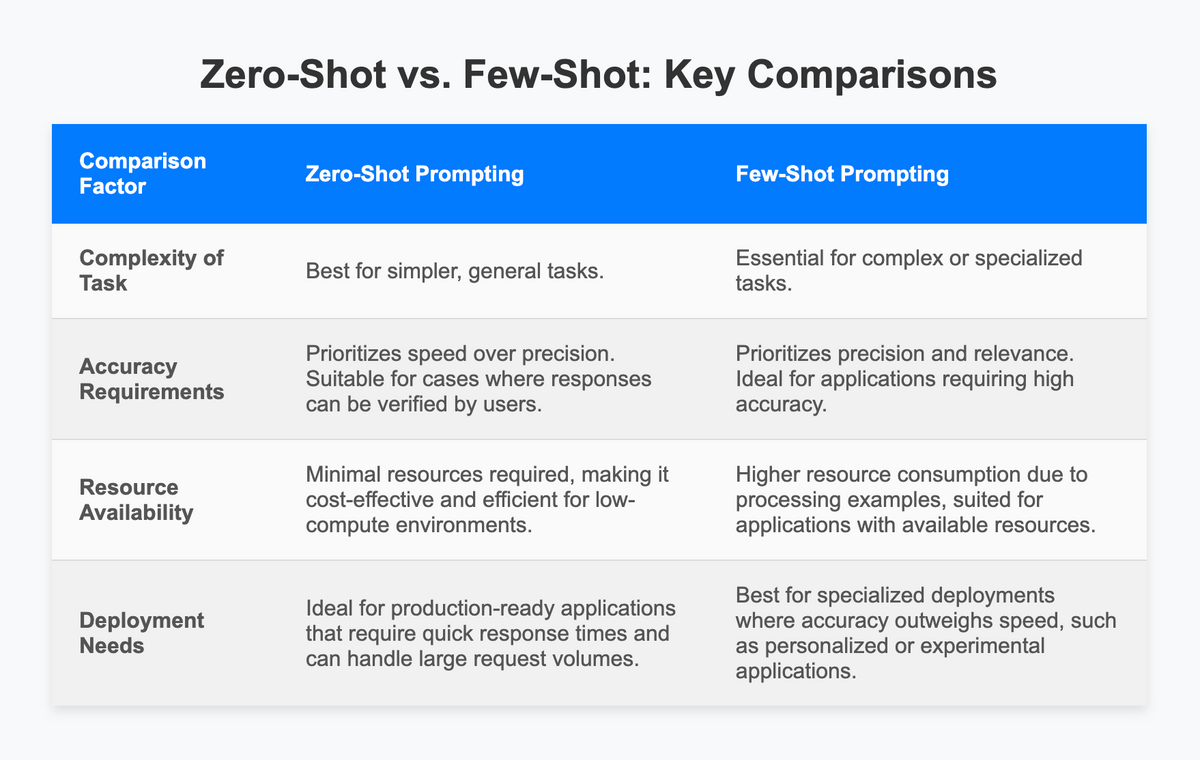
\includegraphics[width=0.85\textwidth]{images/presentacion/table_shots.png}
\end{frame}

\begin{frame}\frametitle{Chain-of-Thought (CoT)}
\begin{columns}[T]
    \column{0.5\textwidth}
    \begin{itemize}
        \item Obliga al modelo a generar pasos intermedios.
        \item Aumenta probabilidad de razonamientos coherentes.
        \item Reduce errores en tareas lógicas y causales.
        \item No es razonamiento real, es secuencialización probabilística.
    \end{itemize}
    \column{0.5\textwidth}
    \centering
    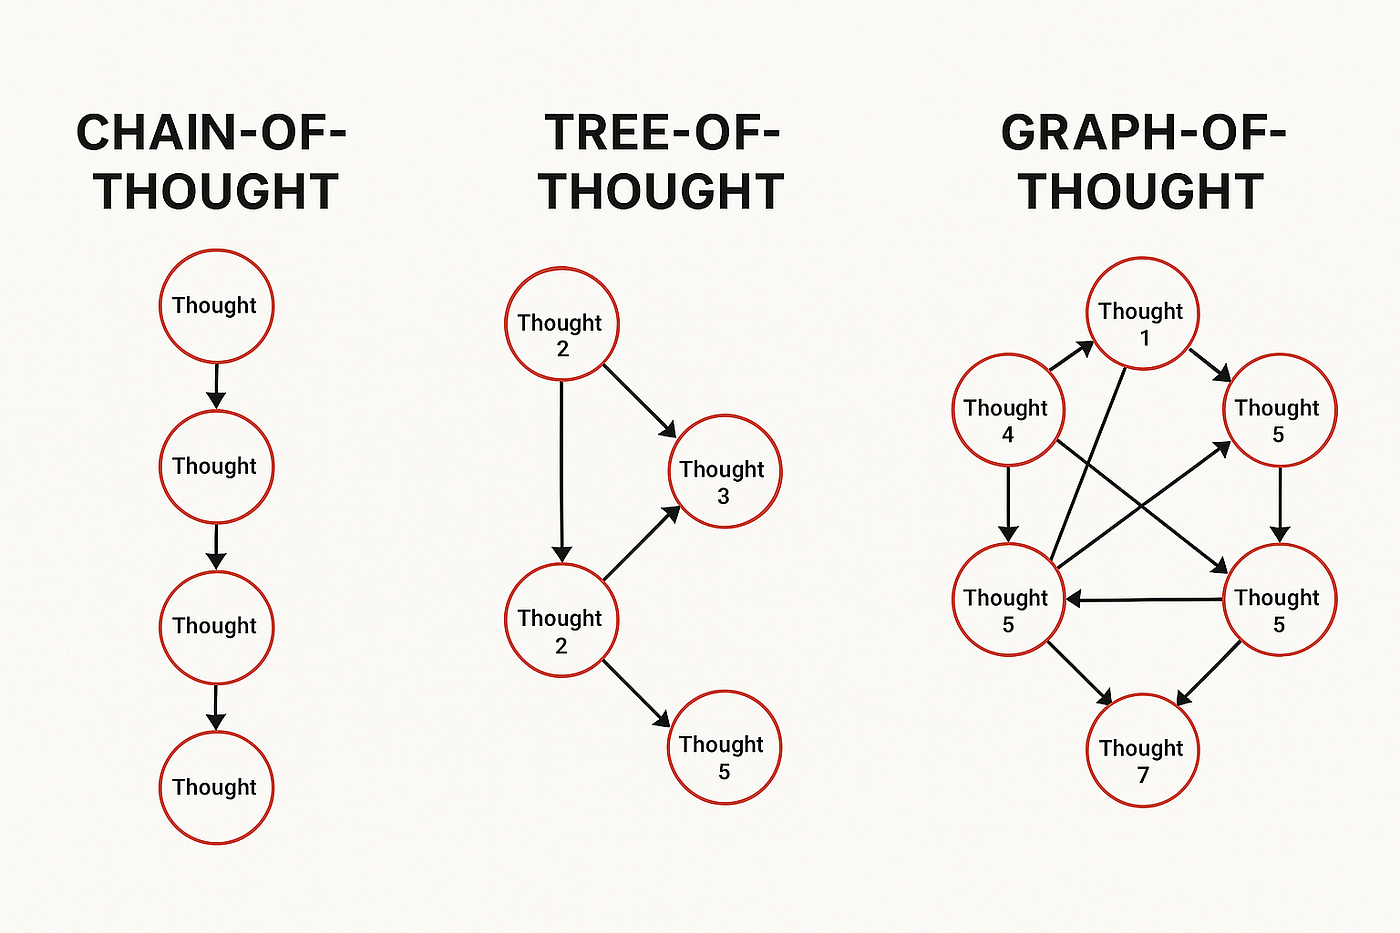
\includegraphics[width=0.8\textwidth]{images/presentacion/cot.png}
\end{columns}
\end{frame}

\begin{frame}\frametitle{Ejemplo CoT en análisis de rendimiento}
\textbf{Pregunta:} ¿Por qué bajó el rendimiento ofensivo?

Modelo debe razonar:
\begin{itemize}
    \item Reducción de minutos.
    \item Menos acciones en último tercio.
    \item Aumento de carga física.
\end{itemize}
\end{frame}

\begin{frame}{Cuándo usar Chain-of-Thought (CoT)}

\textbf{CoT es útil cuando la tarea requiere descomposición lógica o causal:}

\begin{itemize}
    \item \textbf{Diagnóstico de rendimiento deportivo}  
    Identificar causas de variaciones en métricas (minutos, carga, acciones).

    \item \textbf{Evaluación táctica}  
    Analizar secuencias de juego paso a paso para inferir decisiones tácticas.

    \item \textbf{Explicaciones causales}  
    Relacionar eventos: fatiga → menor intensidad → menos acciones decisivas.

    \item \textbf{Razonamiento multi-variable}  
    Cuando intervienen estadísticas físicas, técnicas y contextuales.
\end{itemize}

\textbf{Efecto:} fuerza al modelo a estructurar el proceso antes de la conclusión.
\end{frame}


\begin{frame}{Riesgos de Chain-of-Thought (CoT)}
\textbf{Aunque mejora la coherencia, CoT introduce efectos adversos importantes:}
\vspace{0.5em}
\begin{itemize}
    \item \textbf{Aumento del coste computacional}  
    Generar pasos intermedios incrementa tokens de salida → mayor latencia y coste en sistemas en producción.

    \item \textbf{Ilusión de racionalidad}  
    El modelo puede producir razonamientos estructurados pero incorrectos, dando una falsa sensación de validez.

    \item \textbf{Propagación de errores}  
    Un fallo en un paso intermedio contamina el resto del razonamiento.

    \item \textbf{Mayor exposición a alucinaciones}  
    Cuanto más texto genera el modelo, más oportunidades tiene de introducir información no fundamentada.

    \item \textbf{No aporta verificación factual}  
    CoT mejora forma, no veracidad. No sustituye RAG ni validación externa.

\end{itemize}

\vspace{0.4em}
\textbf{Conclusión:} CoT mejora estructura del razonamiento, pero no garantiza corrección.

\end{frame}


%------------------------------------------------
\section{Errores comunes en Prompt Engineering}
\frame{\sectionpage}

\begin{frame}{Prompts ambiguos}
\textbf{La ambigüedad introduce variabilidad no controlada en la salida del modelo.}
\vspace{0.4em}
\begin{itemize}
    \item No se define con precisión la \textbf{tarea objetivo}.
    \item El modelo debe inferir intención → introduce suposiciones.
    \item Aumenta la \textbf{varianza entre ejecuciones}.
    \item Complica la evaluación automática y la comparación de resultados.
\end{itemize}
\vspace{0.4em}
\textbf{Impacto en sistemas:} salida impredecible → difícil integrar en pipelines.
\textbf{Ejemplo:} “Analiza el partido” → ¿rendimiento físico, táctica, psicología?
\end{frame}


\begin{frame}{Falta de contexto}
\textbf{El modelo no detecta “lagunas”; las rellena probabilísticamente.}
\vspace{0.4em}
\begin{itemize}
    \item Si faltan datos, el modelo usa conocimiento general.
    \item Aumenta riesgo de \textbf{alucinaciones plausibles}.
    \item Se diluye la frontera entre información real e inferida.
    \item En deporte: puede inventar estadísticas, roles o situaciones.
\end{itemize}
\vspace{0.4em}
\textbf{Regla operativa:} lo que no está en el prompt no forma parte de la realidad del sistema.
\end{frame}

\begin{frame}{No controlar el formato de salida}
\textbf{Sin formato definido, la salida es texto narrativo no estructurado.}
\vspace{0.4em}
\begin{itemize}
    \item No se puede validar automáticamente.
    \item Difícil de almacenar y consultar.
    \item No integrable en pipelines Big Data.
    \item Alta variabilidad de estructura entre ejecuciones.
\end{itemize}
\vspace{0.4em}
\textbf{Impacto técnico:} se rompe la trazabilidad del sistema.
\textbf{Solución:} definir siempre esquema de salida (JSON, tabla, claves fijas).
\end{frame}

\begin{frame}{Mezclar demasiadas tareas en un prompt}
\textbf{Un prompt multiobjetivo diluye el foco del modelo.}
\vspace{0.4em}
\begin{itemize}
    \item Clasificar + explicar + evaluar en un solo prompt.
    \item El modelo reparte capacidad entre subtareas.
    \item Respuestas más superficiales y menos precisas.
    \item Mayor probabilidad de incoherencias internas.
\end{itemize}
\vspace{0.4em}
\textbf{Principio de diseño:} un prompt → una tarea principal.
\end{frame}

\begin{frame}{Confiar ciegamente en la salida}
\textbf{La coherencia lingüística no implica veracidad.}
\vspace{0.4em}
\begin{itemize}
    \item Los LLMs son modelos probabilísticos, no sistemas de verificación.
    \item Pueden producir respuestas seguras pero incorrectas.
    \item Mayor riesgo cuando la respuesta parece bien argumentada.
    \item En deporte: decisiones basadas en datos inventados pueden ser críticas.
\end{itemize}
\vspace{0.4em}
\textbf{Requisito de sistema:} validación humana o cruzada con fuentes reales.
\end{frame}

\begin{frame}{No evaluar la calidad de los prompts}
\textbf{Un prompt no evaluado es un componente no controlado del sistema.}
\vspace{0.4em}
\begin{itemize}
    \item Sin métricas no se puede optimizar ni comparar versiones.
    \item Los cambios en prompts afectan al comportamiento global del sistema.
    \item La calidad percibida puede no reflejar estabilidad real.
\end{itemize}
\vspace{0.4em}
\textbf{Resultado:} deriva del sistema sin que se detecte.
\end{frame}

\begin{frame}{Evaluación de prompts en sistemas reales}
\textbf{Un prompt debe evaluarse como cualquier otro componente software.}
\vspace{0.4em}
\begin{itemize}
    \item Consistencia del formato (JSON válido, claves presentes).
    \item Tasa de campos vacíos o incorrectos.
    \item Variabilidad entre ejecuciones con la misma entrada.
    \item Coherencia con datos reales.
    \item Estabilidad tras cambios de modelo o temperatura.
\end{itemize}
\vspace{0.4em}
\textbf{Objetivo:} minimizar varianza y maximizar fiabilidad operativa.
\end{frame}



%------------------------------------------------
\section{Post-training de LLMs}
\frame{\sectionpage}

\begin{frame}\frametitle{Hasta dónde llega el prompting}
\begin{itemize}
    \item Controla formato y tarea.
    \item Reduce ambigüedad.
    \item Mejora consistencia.
    \item Pero no cambia lo que el modelo sabe ni cómo está alineado.
\end{itemize}

\textbf{Por eso existe el post-training.}
\end{frame}

\begin{frame}\frametitle{¿Por qué existe el post-training?}
Un modelo tras el pretraining:
\begin{itemize}
    \item Ha aprendido a predecir texto.
    \item Conoce patrones lingüísticos.
    \item Tiene conocimiento general.
\end{itemize}


Pero:
\begin{itemize}
    \item No está optimizado para seguir instrucciones.
    \item No está alineado con expectativas humanas.
    \item No está diseñado para ser útil como asistente.
\end{itemize}
\end{frame}

\begin{frame}\frametitle{Qué es el post-training}
\begin{itemize}
    \item Conjunto de técnicas que se aplican tras el entrenamiento base.
    \item Objetivo: modificar el \textbf{comportamiento} del modelo.
    \item No enseña nuevo lenguaje, enseña \textbf{cómo responder}.
\end{itemize}

\vspace{0.4em}
\textbf{Idea clave:} transforma un generador de texto en un asistente usable.
\end{frame}

\begin{frame}\frametitle{Ciclo de vida de un LLM}
\begin{center}
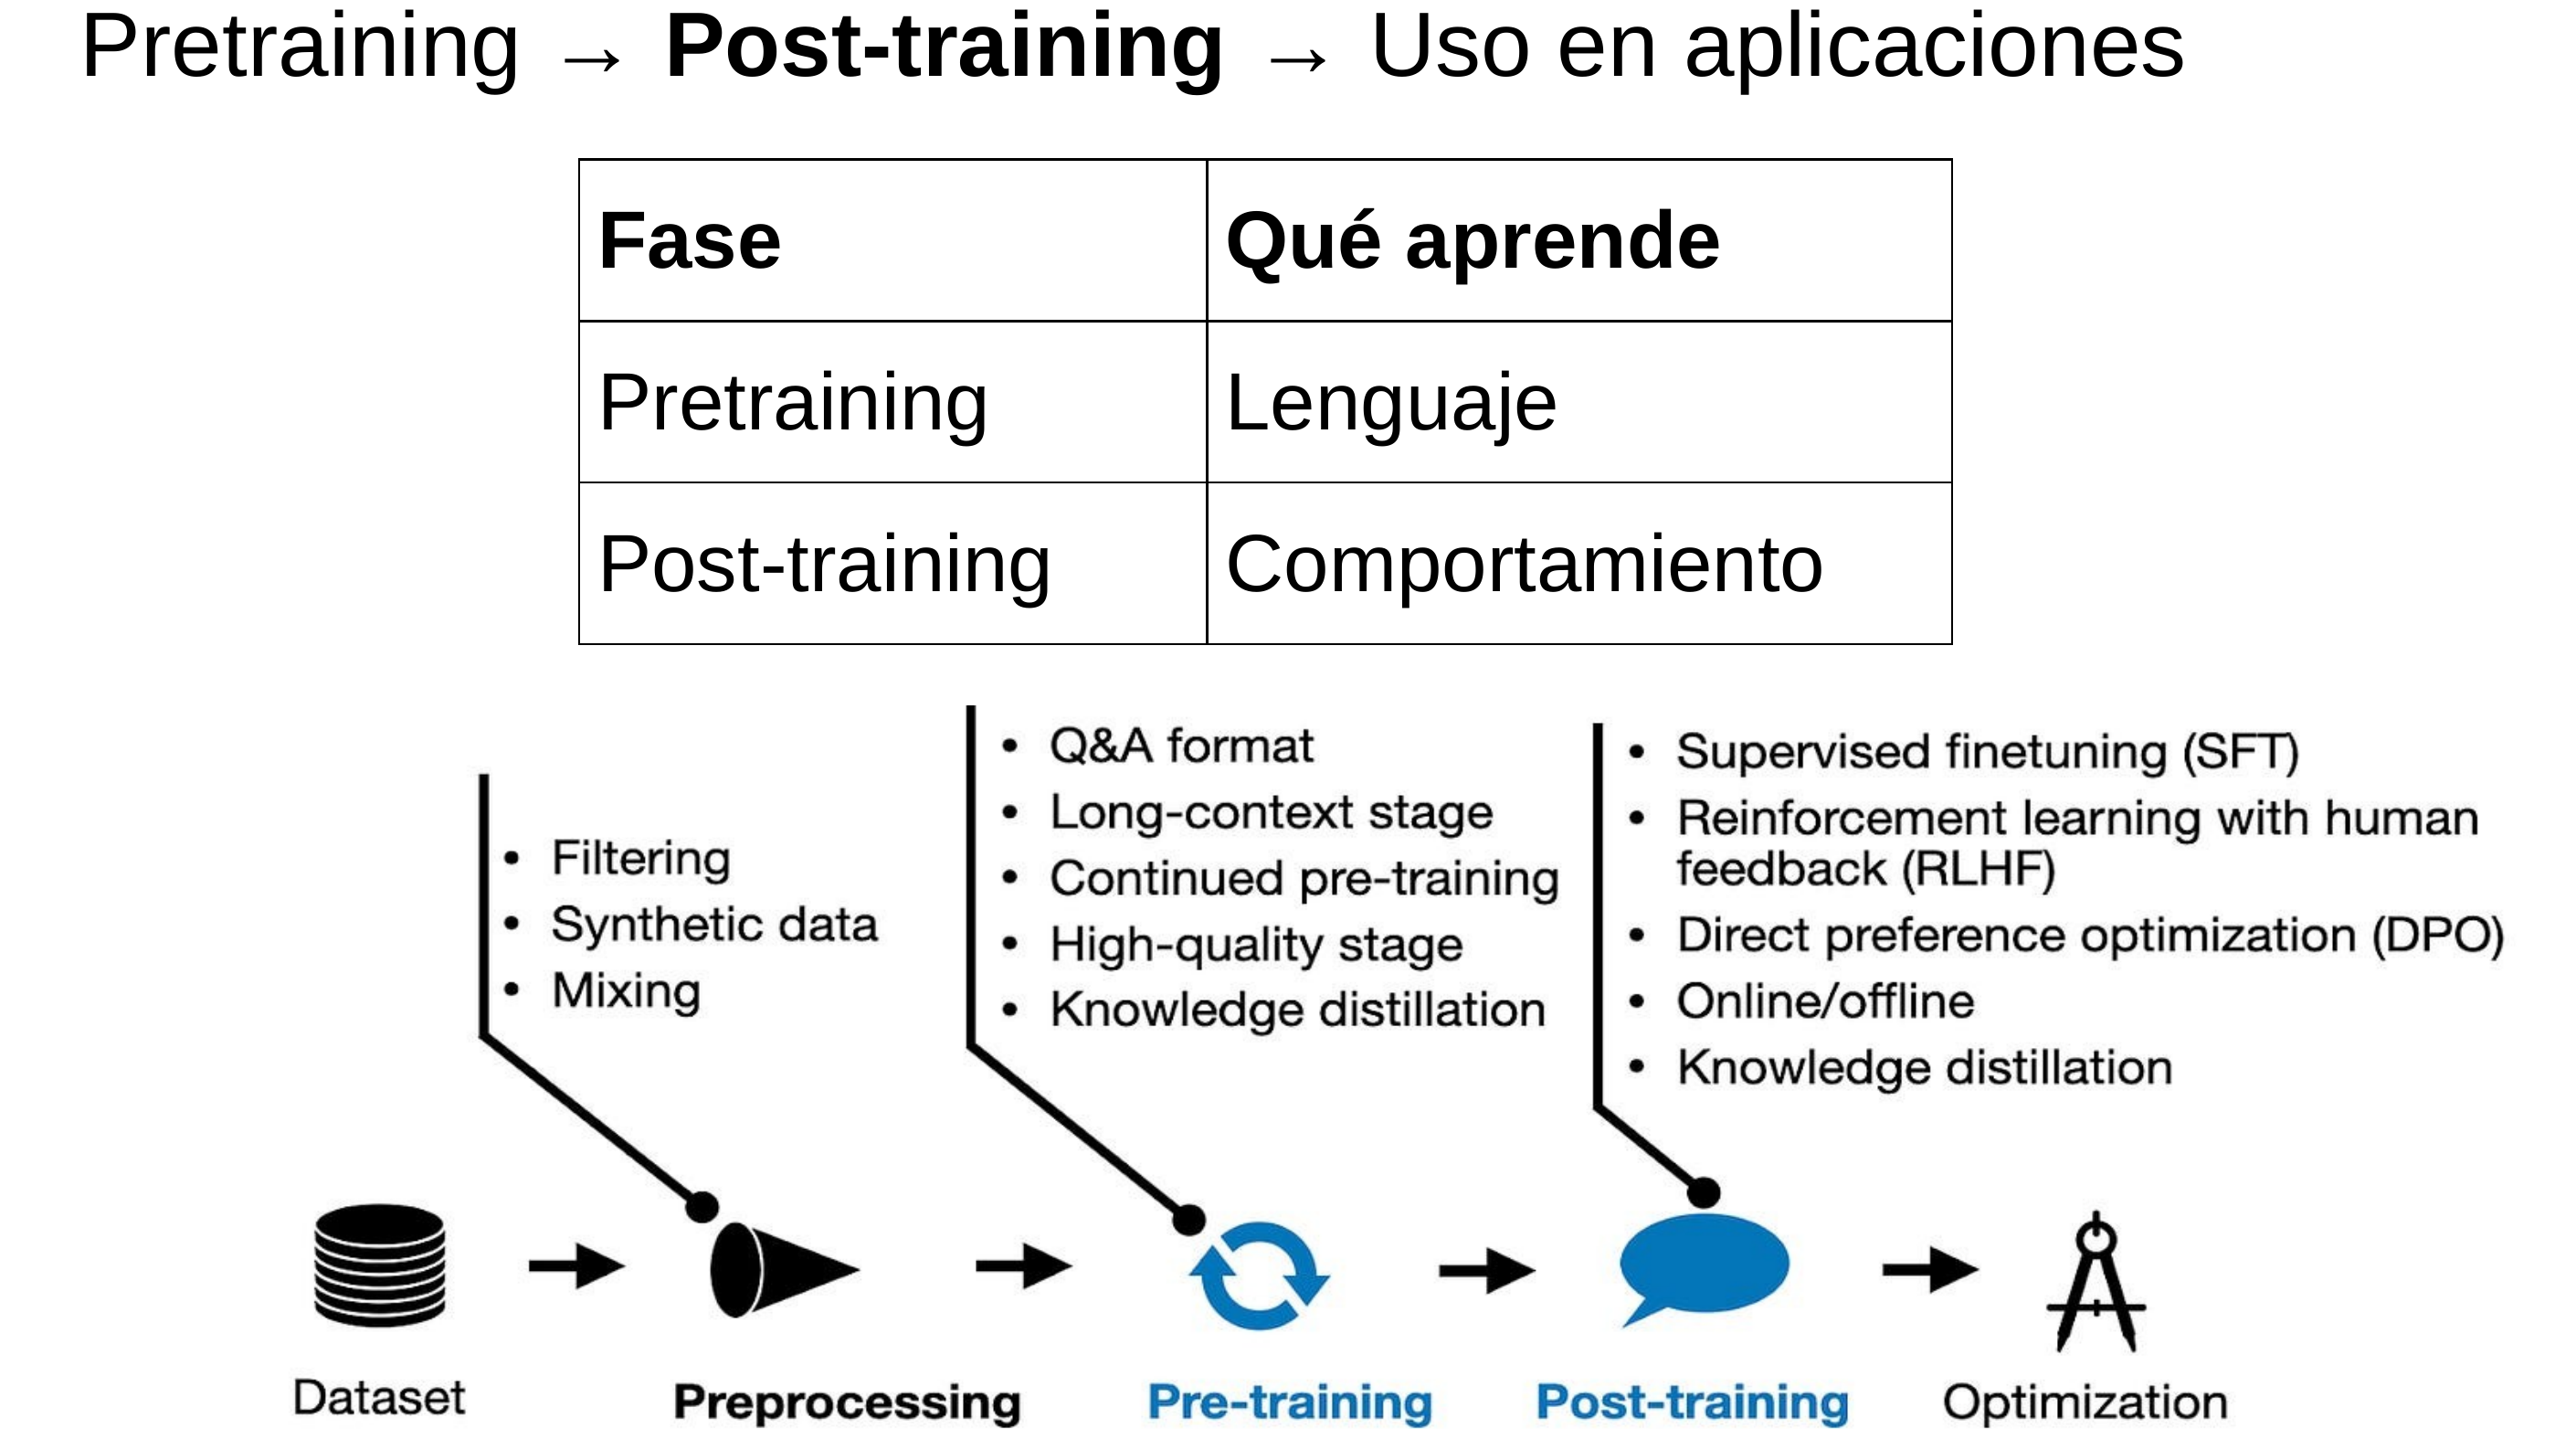
\includegraphics[width=0.8\textwidth]{images/presentacion/pt_lifecycle-07.png}
\end{center}
\end{frame}

\begin{frame}\frametitle{Objetivos del post-training}
\begin{itemize}
    \item Que el modelo siga instrucciones.
    \item Mejorar claridad y estructura de respuestas.
    \item Controlar tono y estilo.
    \item Reducir respuestas peligrosas o inapropiadas.
    \item Enseñar cuándo abstenerse de responder.
\end{itemize}
\end{frame}

\begin{frame}\frametitle{Técnica 1 — Supervised Fine-Tuning (SFT)}
\begin{itemize}
    \item Ajuste con ejemplos humanos correctos.
    \item El modelo imita respuestas bien estructuradas.
    \item Introduce estilo conversacional.
\end{itemize}

\textbf{Limitación:} solo aprende por imitación, no por preferencias.
\end{frame}

\begin{frame}\frametitle{Técnica 2 — Instruction Tuning}
\begin{itemize}
    \item Variante de SFT centrada en seguir instrucciones.
    \item Se entrena con muchas tareas distintas.
    \item Mejora versatilidad del modelo.
\end{itemize}
\textbf{Resultado:} menos necesidad de prompts complejos.
\end{frame}

\begin{frame}\frametitle{Técnica 3 — RLHF}
\begin{itemize}
    \item Reinforcement Learning from Human Feedback.
    \item Humanos comparan respuestas del modelo.
    \item El modelo aprende qué respuestas son preferidas.
\end{itemize}

\textbf{Efecto:} mayor naturalidad y alineación con expectativas humanas.
\end{frame}

\begin{frame}\frametitle{Técnicas modernas: RLAIF y DPO}
\begin{itemize}
    \item RLAIF: feedback generado por modelos IA.
    \item DPO: optimización directa por preferencias.
    \item Más simples y escalables que RLHF clásico.
\end{itemize}
\end{frame}

\begin{frame}\frametitle{Fine-tuning de dominio}
\begin{itemize}
    \item Adaptación a áreas específicas (medicina, derecho, deporte).
    \item Mejora precisión terminológica.
    \item Respuestas más especializadas.
\end{itemize}

\textbf{Riesgo:} pérdida de generalidad y sesgos de dominio.
\end{frame}

\begin{frame}\frametitle{Qué cambia el post-training en la práctica}
\begin{itemize}
    \item El modelo:
    \begin{itemize}
        \item Sigue mejor instrucciones.
        \item Es más conversacional.
        \item Es más prudente.
    \end{itemize}
    \item Pero:
    \begin{itemize}
        \item Sigue siendo probabilístico.
        \item Sigue alucinando.
        \item No tiene acceso a datos externos.
    \end{itemize}
\end{itemize}
\end{frame}

\begin{frame}\frametitle{Relación entre prompting y post-training}
\begin{itemize}
    \item Prompting = control externo.
    \item Post-training = comportamiento interno.
\end{itemize}

\vspace{0.4em}
\textbf{Metáfora:}
\begin{itemize}
    \item Post-training educa al modelo.
    \item Prompting le da instrucciones concretas.
\end{itemize}
\end{frame}

\begin{frame}\frametitle{Limitaciones del post-training}
\begin{itemize}
    \item Alineación imperfecta.
    \item Alucinaciones persistentes.
    \item Puede parecer seguro sin ser correcto.
    \item No sustituye acceso a datos reales.
\end{itemize}
\end{frame}

\begin{frame}\frametitle{Riesgos del post-training}
\begin{itemize}
    \item Modelos demasiado conservadores.
    \item Respuestas genéricas y seguras.
    \item Sesgos heredados del feedback humano.
    \item Puede priorizar parecer correcto sobre ser útil.
\end{itemize}
\end{frame}

\begin{frame}\frametitle{Lecciones aprendidas}
\begin{itemize}
    \item Un LLM no es una fuente de conocimiento.
    \item El prompt es una herramienta de ingeniería.
    \item Las técnicas de prompting mejoran control, no verdad.
    \item El comportamiento base del modelo viene del post-training.
    \item Para trabajar con datos reales necesitaremos RAG.
\end{itemize}
\end{frame}

\end{document}
